%\documentclass[a4paper,man,apacite,floatsintext,donotrepeattitle]{apa6}
\documentclass[a4paper,man,apacite,donotrepeattitle]{apa6}

\usepackage[ngerman, english]{babel}
\usepackage[utf8]{inputenc}
\usepackage{setspace}
\usepackage[table,xcdraw]{xcolor}
\usepackage{pdflscape}
\usepackage{geometry}
\usepackage{amsmath}
\usepackage{footnote}
\usepackage{bm} %bold font in equations
\usepackage[flushleft]{threeparttable} %notes under tables
% For in text revisoins
\usepackage{color}
\newcommand{\revision}[1]{\color{red}{#1}}
%tikz
\usepackage{tikz}
\usetikzlibrary{calc, positioning, shapes, arrows}

\raggedbottom % Formatting

%Title Page
\title{How Response Time Models Should Inform Test Assembly: A Note on the Speed Sensitivity Parameter
\vspace{3cm}}
\shorttitle{Response Time Models in Test Assembly}
\author{\color{white}.}
\affiliation{\color{white}.}

\abstract{
In high-stakes testing, often multiple test forms are used and a common time limit is enforced. Therefore, test fairness requires that all test forms have identical speededness. The hierarchical response time model \cite{vanderLinden.2011reparamet} is a popular tool to control the speededness of test forms. We investigated whether extending this model with a speed sensitivity parameter can aid controlling the speededness of test forms. In an empirical example, the extended model fitted the data better. In a simulation study, test forms with differential speed sensitivity led to substantially different ability estimates, especially for slow test takers with high ability. We therefore recommend the use of the extended model for the calibration of item pools for high-stakes testing.
}

\begin{document}
\maketitle

% ----------------------------- Introduction
\section{Theoretical Background}
In high-stakes assessments like college administration tests (e.g. SAT; \citeNP{SAT.2016}) or language proficiency tests (e.g. TOEFL; \citeNP{ETS.2010}), important consequences result from test scores, such as admission to university or other educational programs. The high-stakes connected to the test outcome have important implications for the design and analysis of the respective tests. First, in order to increase test security, often multiple parallel test forms are used. This prevents cheating during testing sessions with multiple test takers and sharing knowledge about the test by former test takers \cite{Luecht.2011}. Second, for reasons of fairness, testing conditions are standardized across test takers and test occasions. For instance, the time limit for the test is equal regardless of the test form. Third, due to the high-stakes, test takers are often assumed to be highly motivated. Therefore, missing responses are commonly considered informative, that is, they are scored as incorrect responses. This scoring rule is communicated to test takers, to prevent test takers from strategically not responding to items they feel unable to provide a correct response to. Ignoring missing values as a scoring rule could incentivize test takers to omit these items and thereby lead to biased and unfair ability estimates. 

When multiple test forms are used, they are often required to be parallel, which means that both the expected ability estimate $E(\hat{\theta})$ as well as the expected standard error $E(\widehat{SE_{\theta}})$ for all test takers should be independent of the administered test form $z$, so that $E(\hat{\theta} |z) = E(\hat{\theta})$ and $E(\widehat{SE_{\theta}} |z) = E(\widehat{SE_{\theta}})$ hold. When missing responses are scored as incorrect, differences in the speededness of the test forms can violate this requirement\footnote{given that ability and speed are distinct constructs, which recent research has shown to be a reasonable assumption \cite{Partchev.2011, vanderLinden.2009}.}. Imagine one test taker, working at a specific speed, and a test administration with two test forms A and B that only differ in their expected test time for the specific test taker. The time limit for the test administration is 60 minutes and the expected total response time of the test taker on test form A is 60 minutes but 70 minutes on test form B. When confronted with test form B, the test taker has to choose from three strategies:
\begin{seriate}
\item Work with the identical speed as on test form A and not reach the end of the test, 
\item work with the identical speed as on test form A and omit items, or 
\item work with increased speed and respond to all items in time.
\end{seriate}
Missing responses resulting from strategies (a) and (b) are scored as incorrect. Working with increased speed (c) usually leads to decreased accuracy \cite<cf. the within-person speed-accuracy trade-off;>{Goldhammer.2015, Tijmstra.2018}. Hence, all strategies will result in a lower expected ability estimation for the individual on test form B compared to test form A. Combinations of the three strategies are also plausible but will have similar consequences on the ability estimation.

The example illustrates that the speededness of a test is an interaction of the time intensity of its items, the time limit set on the test and the speed the test taker is working with on the test \cite{vanderLinden.2011ATA}. As the speed level usually varies between persons, the degree of speededness of a test can also be expected to vary between persons. A test taker who works fast with a high level of accuracy will score higher on a high-stakes test with a time limit than an equally accurately responding test taker working at a lower speed, which leads to the person to run out of time. Consequently, however, the measured latent construct is no longer a pure ability measure, but a composite measure of speed and ability. Whether this is seen as a conceptual property of the test or a byproduct of the testing conditions differs. In this paper we make no assumptions on the nature of speed differences between persons and to which degree they should affect ability measurement in high-stakes testing. For a discussion of this issue see, for example, the work of \citeA{Tijmstra.2018}. Instead, we focus on how to hold the level of speededness constant across all test forms within each individual test taker. In the following section, we briefly outline the usual test assembly process and the analysis that is commonly performed to obtain individual ability estimates in high-stakes assessments. Based on this we then discuss which approaches can be used to prevent differentially speeded test forms.

\subsection{Assessment Framework}
\subsubsection{Test Assembly}
The common process of creating multiple parallel test forms contains of the following steps \cite{SAT.2016, vanderLinden.2005}: 
\begin{APAenumerate}
\item Developing items 
\item Using items on a piloting sample (Piloting)
\item Item parameter estimation (Calibration)
\item Assembly of items from an item pool to parallel test forms (Test Assembly)
\end{APAenumerate}
Criteria for the assembly of tests, besides test speededness, include the test information function, comparability of content, and similar distribution of item types \cite{vanderLinden.2005}. Due to the emergence of computer-based testing, balancing speededness has become substantially easier. In this paper we assume that response times are available from a computer-based conducted piloting study. 

\subsubsection{Ability Estimation}
For the estimation of latent abilities an often used choice is the 2PL model. As already described, we assume that missing responses are scored as incorrect. Throughout this paper we adopt the notation of \citeA{Fox.2010}, denoting items as $k = 1, ..., j$ and persons as $i = 1, ...., n$. In the 2PL model, the probability to solve an Item $k$ correctly can be denoted as:  

\begin{equation}
	P(y_{ik} = 1|\theta_{i}, a_{k}, b_{k}) = \frac{exp(a_{k}\theta_{i} - b_{k})} 
							{1 + exp(a_{k}\theta_{i} - b_{k})}.
	\label{eq:2PL}
\end{equation}  

\subsection{Balancing Speededness}
Several strategies have been proposed to balance speededness across the test forms of a test administration, for example using observed response times from a piloting study \cite<e.g.,>{vanderLinden.2005}. In the following section, we discuss the current state of the art approach, which uses response time modeling via the hierarchical response time model, rather than observed response times.

\subsubsection{Hierarchical Response Time Model}
Recently, \citeA{vanderLinden.2011reparamet} proposed the use of the \textit{hierarchical response time model} (HRT) \cite{vanderLinden.2006} for balancing speededness across test forms. First, we will briefly describe the HRT in general and then discuss how this model can be used to control the speededness of test forms. 

\begin{figure}
\begin{center}
	\begin{tikzpicture}[scale = 2.4]

\tikzstyle{arrow} = [thick,->,>=stealth, line width=0.5pt];

\node(sumI) [draw, circle] at (1,1.1) {$\sum_{k}$};

\node(ab) [draw, circle] at (0.5,0.5) {a, b};
\node(lambda) [draw, circle] at (1.5,0.5) {$\lambda$};

\node(Y) [draw, rectangle] at (0.5,0) {Y};
\node(T) [draw, rectangle] at (1.5,0) {RT};

\node(theta) [draw, circle] at (0.5,-0.5) {$\theta$};
\node(zeta) [draw, circle] at (1.5,-0.5) {$\zeta$};

\node(sumP) [draw, circle] at (1,-1.1) {$\sum_{i}$};

\node(IRT) [] at (0.5,-1.4) {IRT model};
\node(RT) [] at (1.5,-1.4) {RT model};

\node(lvl2a) [] at (2.5,1.1) {Level 2};
\node(lvl1) [] at (2.5,0) {Level 1};
\node(lvl2b) [] at (2.5,-1.1) {Level 2};

\draw [arrow] (sumI) -- (ab);
\draw [arrow] (sumI) -- (lambda);

\draw [arrow] (theta) -- (Y);
\draw [arrow] (ab) -- (Y);
\draw [arrow] (zeta) -- (T);
\draw [arrow] (lambda) -- (T);

\draw [arrow] (sumP) -- (theta);
\draw [arrow] (sumP) -- (zeta);

\draw[dashed] (Y) ellipse (0.4cm and 0.8cm);
\draw[dashed] (T) ellipse (0.4cm and 0.8cm);

\draw[dotted] (0,0.8) -- (2,0.8);
\draw[dotted] (0,-0.8) -- (2,-0.8);

	\end{tikzpicture}	
	\end{center}
\caption[alt caption]{Structure of the Hierarchical Response Time Model \cite{KleinEntink.2009CDM}.}
\label{fig:HRT}
\end{figure}

The HRT jointly models responses and response times (Figure \ref{fig:HRT}), assuming lognormal distributed response times. The measurement model of the HRT for responses times $RT_{ik}$ can be written as 
\begin{equation}
	\ln RT_{ik} = \lambda_{k} - \zeta_{i} + \epsilon_{ik}, 
	\quad \textrm{with} \quad \epsilon_{ik} \sim N (0, \sigma^2_{\epsilon_{k}}).
	\label{eq:HRT}
\end{equation}
$\lambda_{k}$ represents the average time it takes to work on an specific item (\textit{item time intensity}), while $\zeta_{i}$ represents the average speed with which a person works (\textit{person speed parameter}). Note that, compared to the traditional IRT model for accuracy, the direction of the item difficulty and person parameter are reversed. Hence, a lower person speed parameter leads to higher expected response times while a lower item time intensity parameter leads to lower expected response times. In addition, an item-specific residual variance $\sigma^2_{\epsilon_{k}}$ is estimated. All item parameters\footnote{Note that \citeA{vanderLinden.2006} also includes the inverse of the residual variance $\sigma^2_{\epsilon_{k}}$ in the joint item parameter distribution. For better comparability with the later described model we slightly modify the HRT by assuming a univariate distributed item specific residual variance, independent from the distribution of the other item parameters.} and the two person parameters as in Equations \ref{eq:2PL} and \ref{eq:HRT} are assumed to stem from joint multivariate normal distributions with

\begin{equation}
	(a_{k}, b_{k}, \lambda_{k}) \sim \mathcal{N}(\bm{\mu_{I}}, \bm{\Sigma_{I}})
	\label{eq:HRT_ItemMVN}
\end{equation}
\begin{equation}
	(\theta_{i}, \zeta_{i}) \sim \mathcal{N}(\bm{\mu_{P}}, \bm{\Sigma_{P}}).
	\label{eq:gHRT_PersonMVN}
\end{equation}
 
In his paper, \citeA{vanderLinden.2011reparamet} proposed balancing the item parameters $\lambda_{k}$ and $\sigma^2_{\epsilon_{k}}$ across test forms and showed that this approach performed better than using observed response times to balance speededness across test forms, as it for example also controls for differing variances in response times between items.

However, there is still an important issue with respect to the presented response time model-based approach. The HRT allows items to have different intercept parameters $\lambda_{k}$ and different residual variances $\sigma^2_{\epsilon_{k}}$. Indeed, \citeA{vanderLinden.2006} even introduces the inverse of the residual variance as the discrimination parameter\footnote{Labeling the inverse of the residual variance as a discrimination parameter has also led to some confusion in the literature. For example \citeA{Bertling.2018} cite \citeA{vanderLinden.2006} but introduce the model with $\alpha_k$ as a slope parameter instead of the inverse of the residual variance.} $\alpha_k$: 

\begin{equation}
	\alpha_k = \frac{1}{\sigma^2_{\epsilon_{k}}}.
	\label{eq:HRT_discr}
\end{equation}

The parameter thereby represents the precision of the response time distribution \cite{Molenaar.2015.gLIRT}. However, compared to models from confirmatory factor analysis, the HRT resembles a tau-equivalent measurement model \cite[pp. 236-252]{Brown.2006}, or compared to IRT models, it resembles a 1PL model \cite<e.g.>{deAyala.2009}. These models have in common that they lack a slope parameter and therefore, speaking in terms of more generalized models, assume that the slope parameter is equal across all items or indicators. This equals the assumption that all manifest indicators of the measurement model correlate equally strong with the measured latent construct. Conceptually speaking for response time modeling, this means that the HRT assumes that items do not differ in their sensitivity to speed differences across persons. 

In this paper, however, we will argue that items can differ in the extent to which they are sensitive to speed differences, and that this variability across items needs to be taken into account when assembling test forms that should have equal speededness for each test taker. In the next section, we will discuss the generalized Hierachical Response Time Model \cite{Fox.2007} which allows differences in speed sensitivity across items by introducing a slope parameter into the response time measurement model. 

\subsubsection{Generalization of the Hierarchical Response Time Model}
\citeA{Fox.2007} and \citeA{KleinEntink.2009} proposed a generalization of the Hierarchical Response Time model which we call the \textit{generalized hierarchical response time model} (gHRT). It introduces a slope parameter called $\phi_{k}$ into the measurement model for response times. The measurement model of the gHRT is comparable to the 2PL model in IRT \cite<e.g.>{deAyala.2009} or the congeneric measurement model in confirmatory factor analysis \cite[pp. 236-252]{Brown.2006}: 
\begin{equation}
	\ln RT_{ik} = \lambda_{k} - \phi_{k} \zeta_{i} + \epsilon_{ik}, 
	\quad \textrm{with} \quad \epsilon_{ik} \sim N (0, \sigma^2_{\epsilon_{k}}),
	\label{eq:gHRT}
\end{equation}
with the joint item distribution 
\begin{equation}
	(a_{k}, b_{k}, \lambda_{k}, \phi_{k}) \sim \mathcal{N}(\bm{\mu_{I}}, \bm{\Sigma_{I}}).
	\label{eq:gHRT_ItemMVN}
\end{equation}

Conceptually, the parameter $\phi_{k}$ allows for individual items being more sensitive to speed differences between test takers than other items. To avoid confusion with the $\alpha_k$ parameter that  \citeA{vanderLinden.2006} labels as a discrimination parameter in the HRT, we will use the term \textit{speed sensitivity} to refer to $\phi_{k}$ throughout this paper. 

To illustrate the difference between the discrimination parameter introduced by \citeA{vanderLinden.2006} and the speed sensitivity parameter of the gHRT, Figure \ref{fig:discr_diff} shows the  expected response time distributions for two persons with differing speed levels on three different items. The black lines represent the expected response time distribution for a fast person with $\zeta_1 = 1$, the grey lines represent the expected response time distribution for a slow person with $\zeta_2 = -1$. The left graph shows the expected response time distributions for an item with a low $\alpha_k$ parameter (and therefore a high residual variance) and a low speed sensitivity $\phi_k$. The graph in the middle shows the consequences for the expected response time distributions if the $\alpha_k$ parameter increases (which means the residual variance decreases). The graph on the right shows the consequences if the $\phi_k$ parameter  increases. The graphs show that the $\alpha_k$ parameter controls the variance around the mean expected response times (and is strongly connected to the concept of reliability), while $\phi_k$ controls how far the means of the expected response time distributions differ between persons with differing speeds.

\begin{figure}
	\begin{center}
	 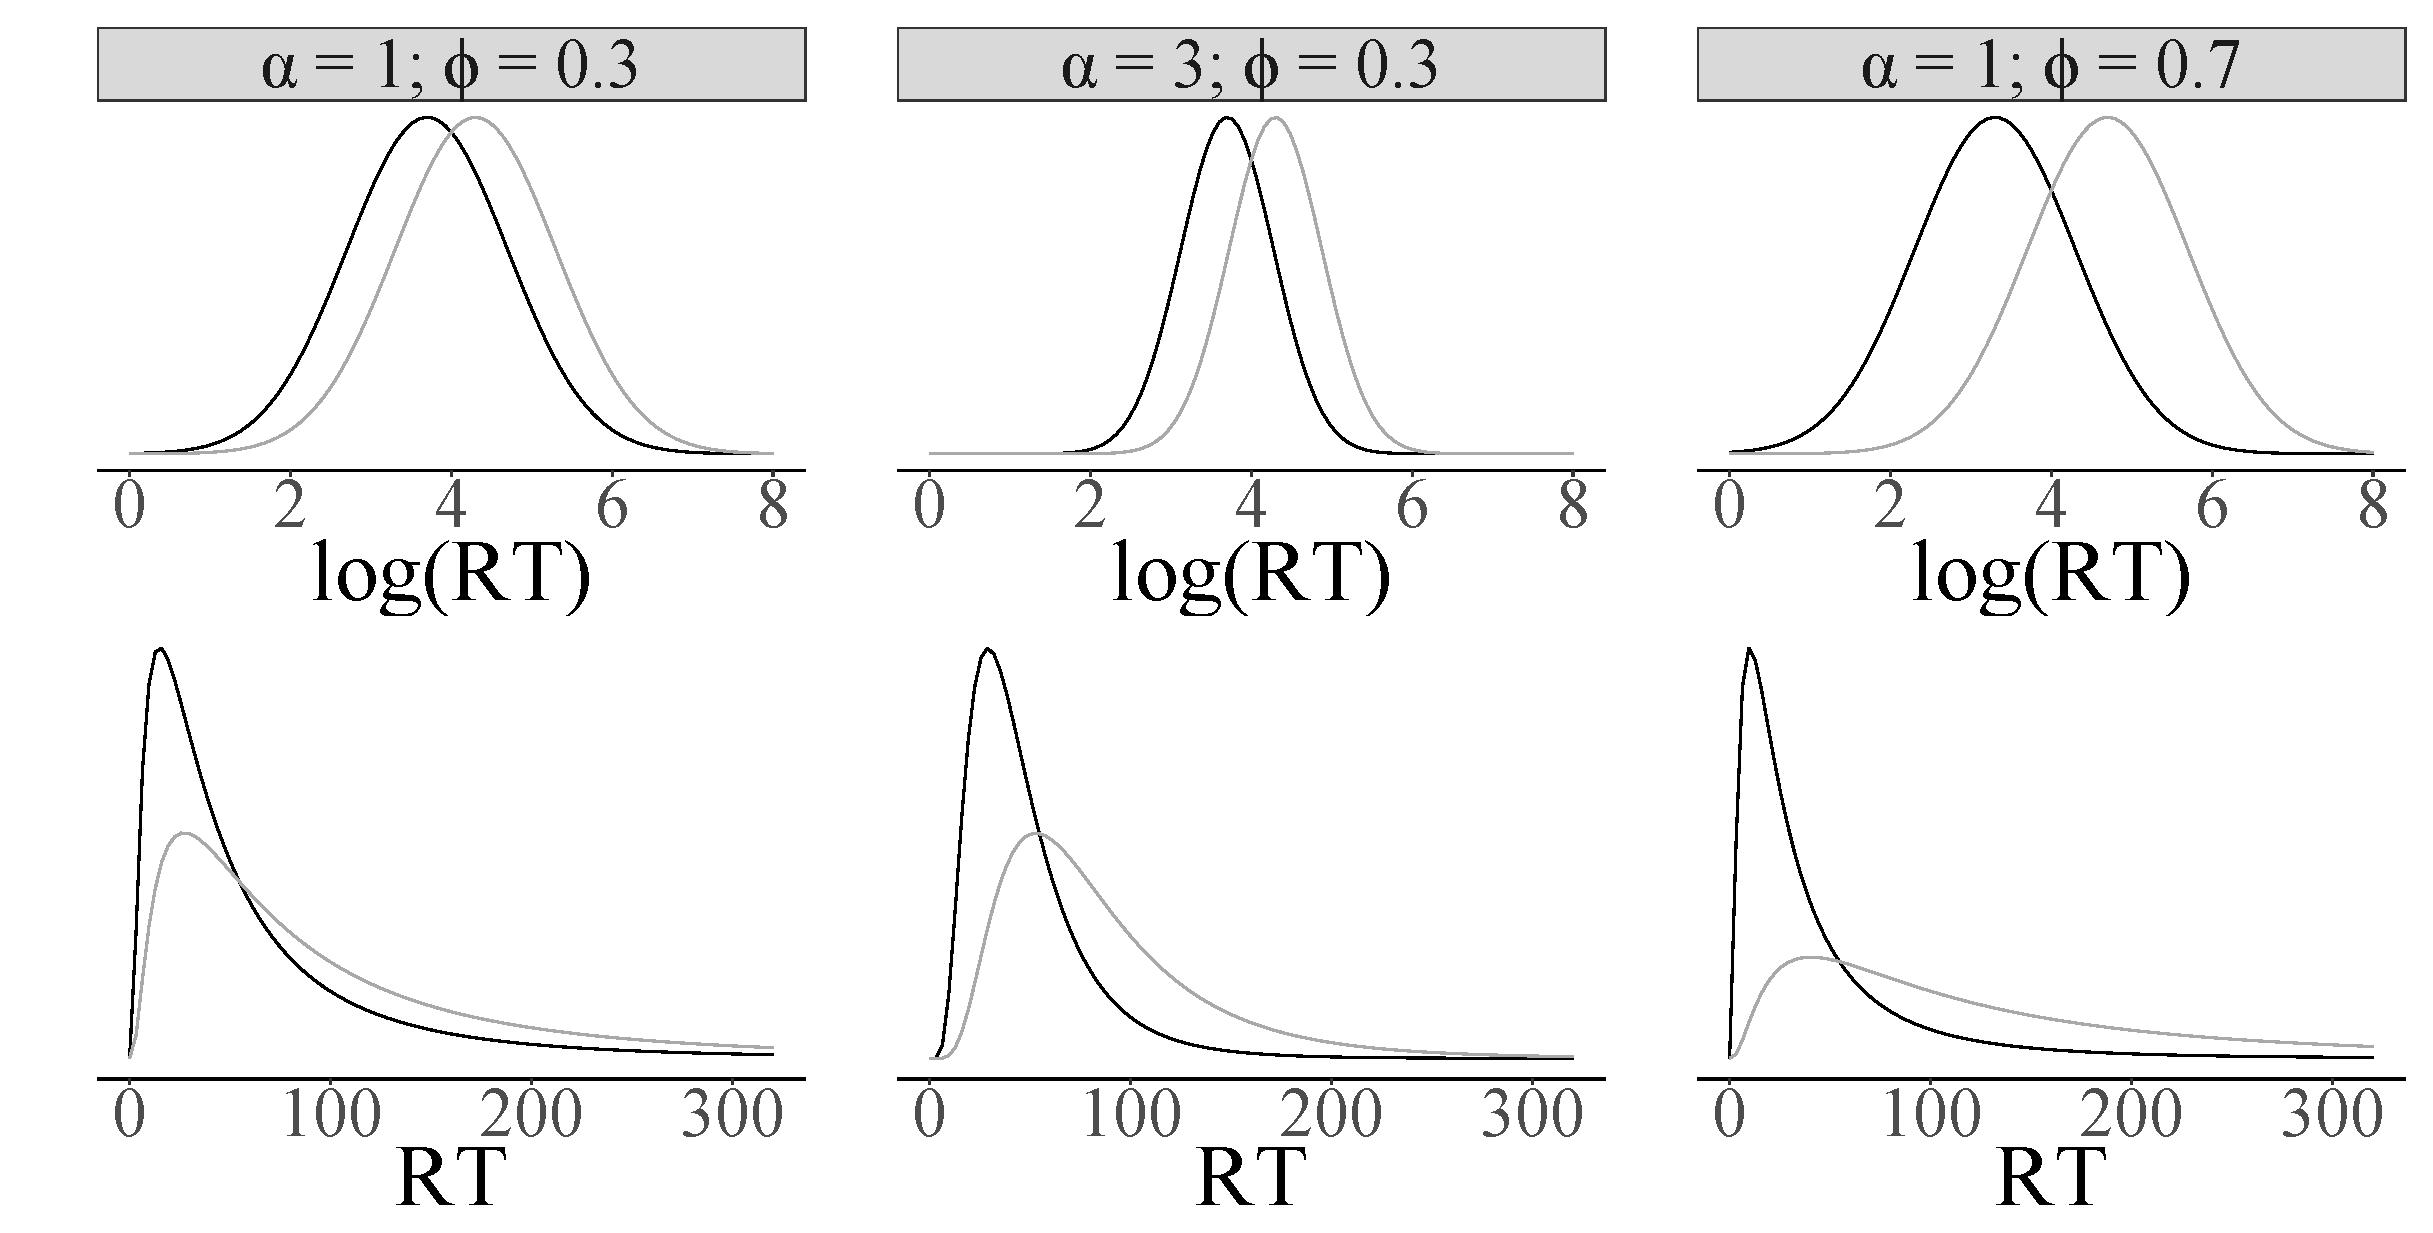
\includegraphics[height = 0.30\textheight]{discrimination_comp.eps}
	\end{center}		
	 \caption{Expected log response time (upper row) and response time (lower row) distributions of a fast person with $\zeta_1 = 1$ (black line) and a slow person with $\zeta_2 = -1$ (grey line) on three different items, all with $\lambda_k = 4$.} 
	 \label{fig:discr_diff}
\end{figure}

As the speed sensitivity parameter is the main focus of the current paper, we would like to illustrate its conceptual meaning by an example: Assume there are two math items in a test with equal time intensity ($\lambda_1 = \lambda_2 = 4$) but with different speed sensitivity parameters ($\phi_1 = 0.3$; $\phi_2 = 0.7$). The first item is a simple task embedded in a long text, while the second requires a lengthy calculation. It seems plausible to assume that the second item is more sensitive to working speed specific to math items, because the calculation is longer. In contrast, the first item could be less sensitive to mathematical working speed, because the response time mostly depends on the reading speed. As reading and mathematical literacy are assumed to be distinct constructs, this is plausible also the case for reading and mathematical speed. The consequences for the Response Time Characteristic Curve, as also described in \citeA{Fox.2010}, can be seen in Figure \ref{fig:phi_theoret}.

\begin{figure}
	\begin{center}
	 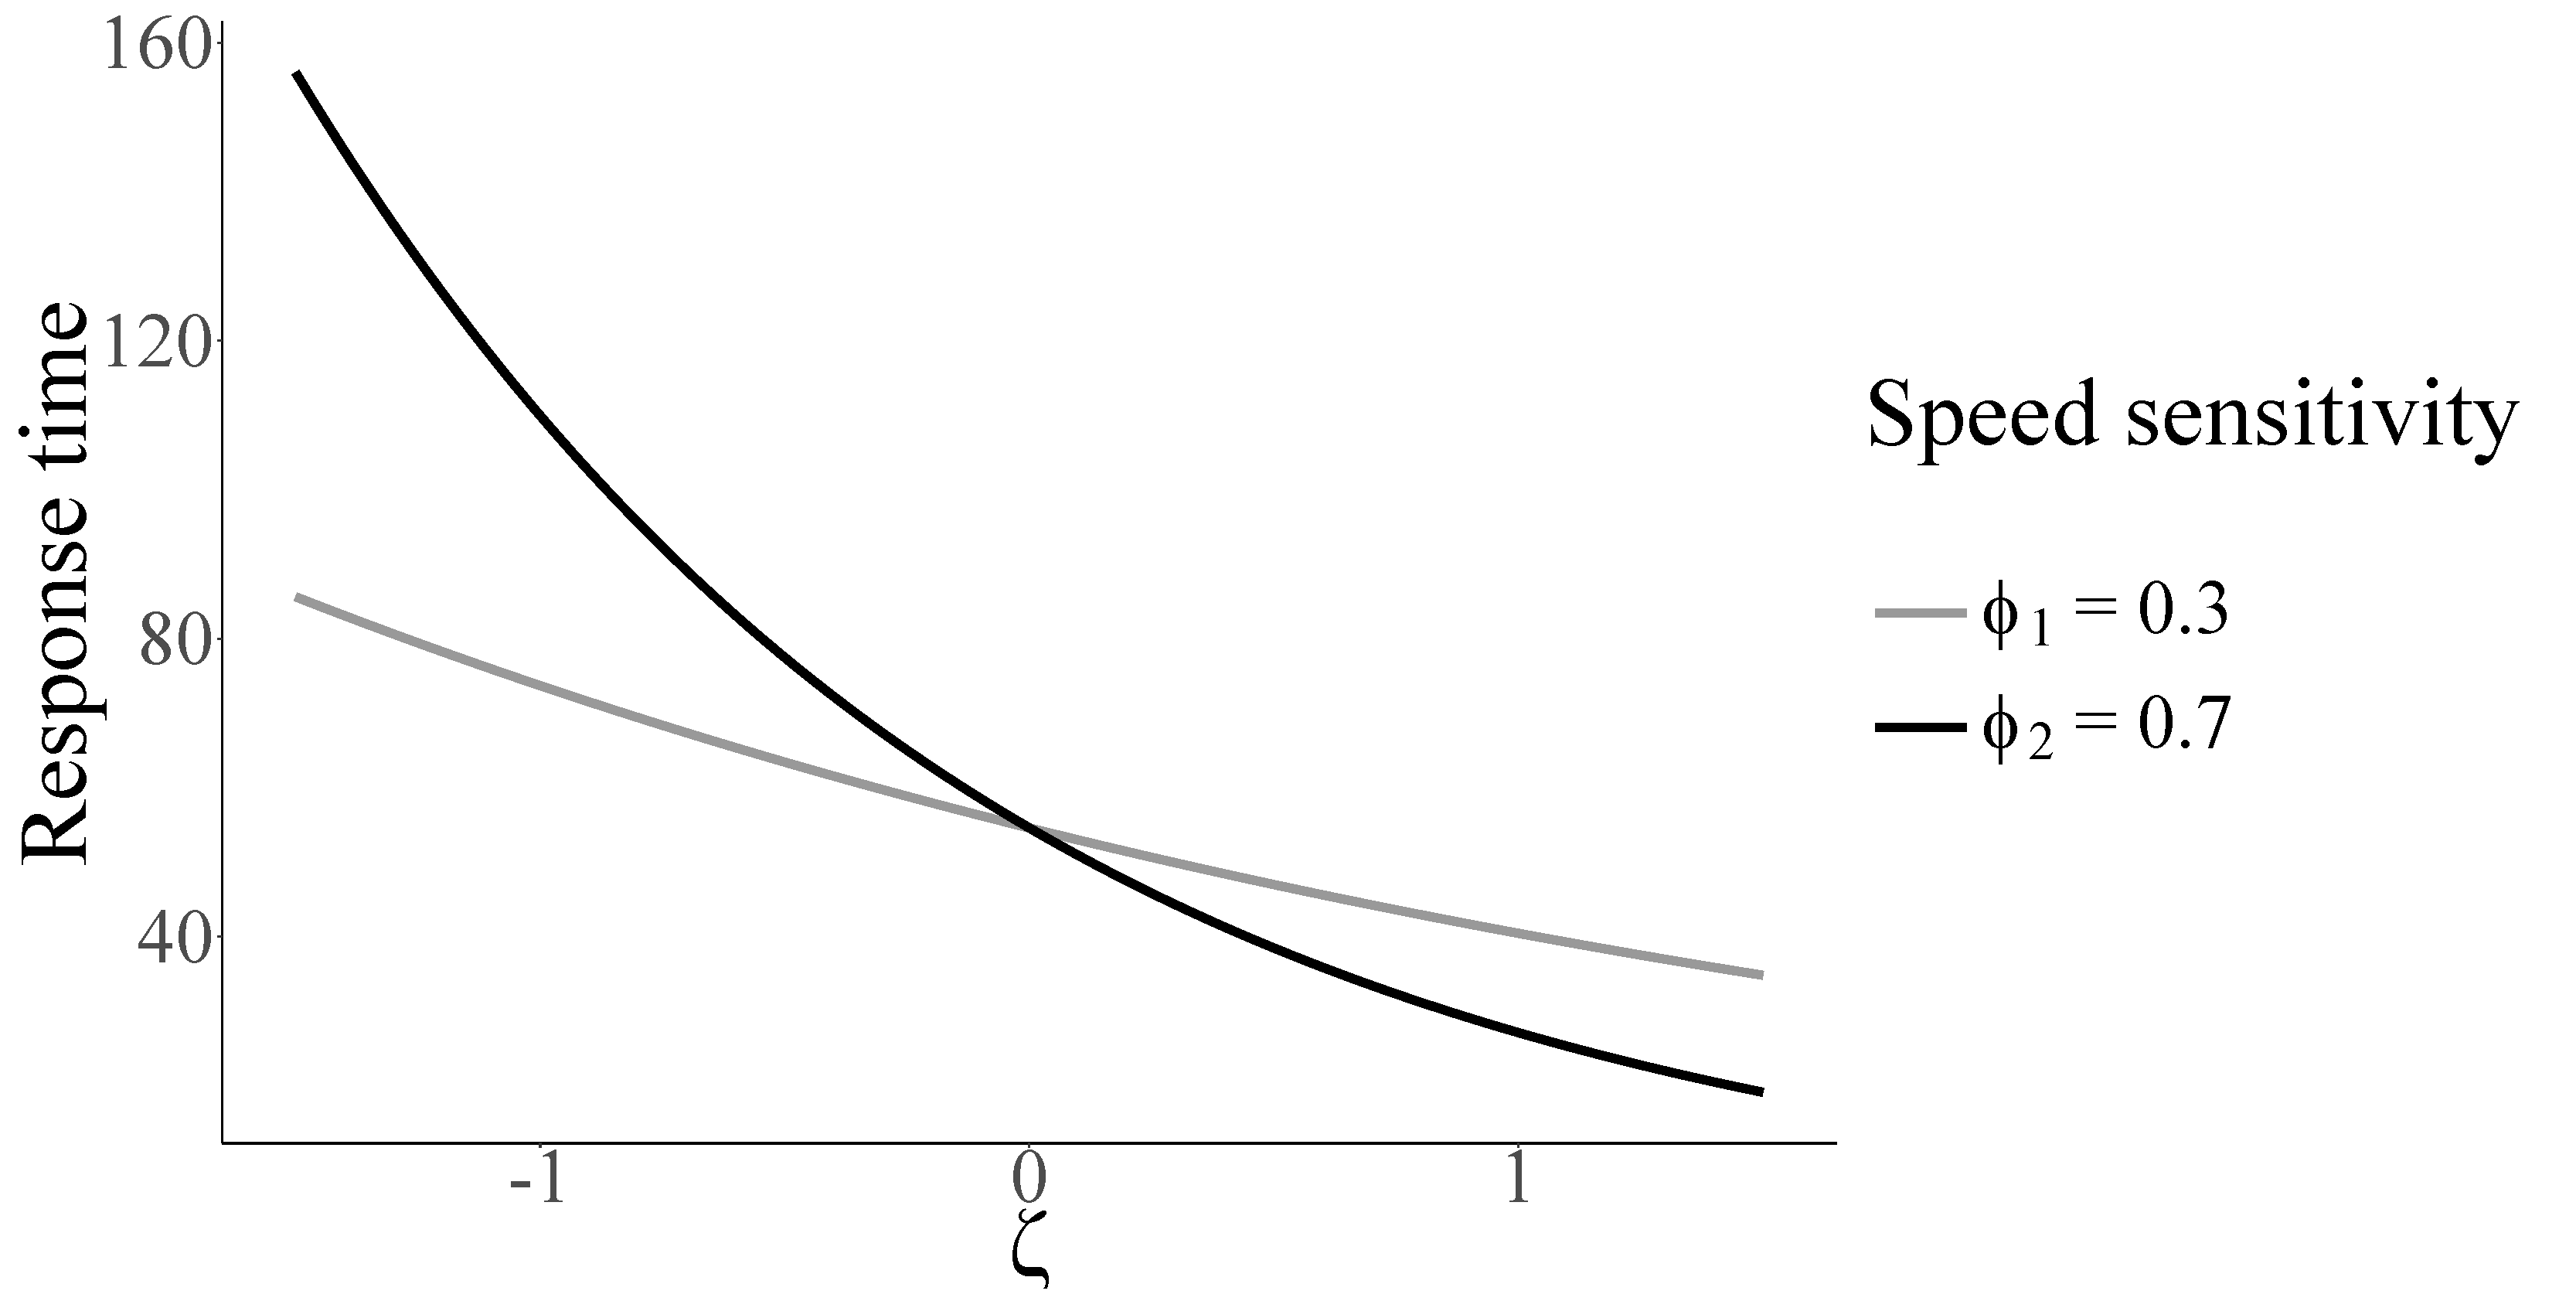
\includegraphics[height = 0.25\textheight]{phi_theoret.eps}
	\end{center}		
	 \caption{Response Time Characteristic Curve of two items with identical time intensity ($\lambda_{k} = 4$) and differing item speed sensitivity parameters $\phi_{k}$.}
	 \label{fig:phi_theoret}
\end{figure}

As Figure \ref{fig:phi_theoret} shows, differences in expected response times between two items with identical time intensity but with different speed sensitivity vary depending on the person speed level $\zeta$. Differing speed sensitivities will not lead to differences in response times for medium speed levels ($\zeta_{k}$ = 0) but to substantial differences for slow ($\zeta_{k}$ = -1) and fast test takers ($\zeta_{k}$ = 1), with differences increasing with increasing deviation from $\zeta_{k}$ = 0. For a test-taker with $\zeta_i = -1$ the expected response times of the two example items are 73.70 and 109.95 seconds. As time pressure usually only occurs for slow participants, generally only differences in response times for slow but not for fast participants will be relevant for the estimation of ability in educational assessments. 

Therefore the questions arise, whether
\begin{seriate} 
\item the gHRT fits empirical data better than the HRT and, if this is the case,
\item what the consequences would be for ability estimation in high-stakes assessments. 
\end{seriate}
To our knowledge the HRT and the gHRT have not been compared using data from educational competence tests. Moreover, there have only been a few comparisons of the HRT and the gHRT using empirical data at all, so far focusing on intelligence tests \cite{Goldhammer.2011}, complex problem solving tasks \cite{Scherer.2015}, and mental rotation tasks \cite{Debelak.2014}. However, in all three studies the gHRT showed better fit than the HRT according to the DIC \cite{Spiegelhalter.2002}. In addition, the gHRT has been applied to non-educational vocational credentialing high-stakes data \cite{Fox.2017} and low-stakes data of chess tasks \cite{Fox.2016}. In both cases substantial variance in the speed sensitivity parameter was found across the items. Because these previous studies provide general evidence for the plausibility of the gHRT but the contexts are all rather different from educational assessments, we decided to conduct some empirical data analysis ourselves, using data from an educational assessment. In the section 'Empirical Data Analyses' we describe this procedure, compare the fit of the gHRT and the HRT, and investigate whether items differ in their speed sensitivity.

If the appropriateness of the gHRT indeed holds in educational competence testing and items vary in their speed sensitivity, those differences may also accumulate over test forms of educational high-stakes assessments, when test forms are assembled from an item pool. This could result in test forms that, despite having equal time intensities and similar average observed response times, differ in their sensitivity to speed differences and therefore in their conditional distributions of expected testing times. Especially the substantial differences in expected response times for slow test takers would be important, as they could lead to differences in ability estimates across test forms.  In the section 'Simulation Study', we investigate and describe the possible consequences of unbalanced test forms on ability estimation using simulated data from test forms with item properties as found in the empirical example.


% ----------------------------- Empirical Data Analysis
\section{Empirical Data Analysis}
\subsection{Data Description}
We used the Canadian subsample of the Programme of International Student Assessment (PISA) from 2015 for applications of the HRT and the gHRT. The PISA assessment is an educational large-scale assessment conducted in 72 countries testing 15-year-old students \cite{PISA.2015tech}. The Canadian subsample was chosen because it is the largest sample among all participating countries. The measured competencies were science, mathematics, reading, financial literacy, and collaborative problem solving and the test was administered on computers in most of the participating countries. We chose the PISA data set because the measured competences closely resemble the competences often measured in educational high-stakes assessments and because responses and response times on item level are publicly available. To avoid substantial numbers of missing responses by design, we only used the data for a single test booklet and for all test-takers who worked on this booklet. In PISA 2015, every test form consisted of four booklets and booklets were assembled to a whole of 66 different test forms in the computer-based version. Returning to items within an booklet was only possible within the items sharing a common stimulus and otherwise prohibited. Response times were accumulated across multiple visits of the same item \cite[pp. 45-47]{PISA.2015tech}. We chose the first math booklet (labeled as 'M01'), which appeared in overall eight different test forms, at every position twice. For simplicity, we dichotomized three polytomous items, scoring fully correct responses as correct and partially incorrect responses as incorrect. This resulted in a data set of $j = 12$ dichotomous items and $n = 1863$ persons.  

\subsection{Methods}
The software JAGS \cite{Plummer.jags} and R \cite{R} together with the package rjags \cite{Plummer.rjags} were used for model estimation. We used both the HRT and the gHRT to analyze the data set. In the actual analysis of the PISA data set omitted responses are scored incorrect and number of not reached responses is used as a manifest variable in the background model for the plausible value generation \cite{PISA.2015tech}. Because the aim of this empirical example is the unbiased estimation of item parameters, we chose to ignore all missing values, which is the recommended practice for estimating item parameters \cite{Finch.2008}. Ideal circumstances for piloting and calibrating items are further discussed at the end of this paper. The DIC was calculated and compared between the two models to assess model fit \cite{Spiegelhalter.2002}. The posterior distributions of item parameter means, standard deviations and correlations with other item parameters were investigated. 

\subsubsection{Priors}
Priors were uninformative and chosen in correspondence to \citeA{Fox.2010}. We used a multivariate normal distribution as a prior distribution for the person ability and person speed parameters. An inverse Wishart distribution was used as a hyperprior for the distribution of the three ($b_{k}$, $a_{k}$, $\lambda_{k}$) or respectively four item parameters ($b_{k}$, $a_{k}$, and $\lambda_{k}$, and $\phi_{k}$). For the residual variance $\sigma^2_{\epsilon_{k}}$ a lognormal distribution was used. 

\subsubsection{Model identification}   
The model was identified by fixing the hyperpriors of the person ability and person speed distributions. The means of the person parameter distributions were fixed to 0 ($M_{\theta_{i}} = 0$ and $M_{\zeta_{i}} = 0$), and the variance of the ability was fixed to 1 ($Var_{\theta_{i}} = 1$). For the gHRT the variance of the person speed was also fixed to 1 ($Var_{\zeta_{i}} = 1$). All item parameters were estimated freely. In addition, we also used an alternative identification for the response time measurement model of the gHRT, setting the product of all $\phi_{k}$ to $1$ and estimating the variance of the person speed parameter freely. This identification is, for example, used by \citeA{Fox.2016, Fox.2017} and also implemented in the R package LNIRT by \citeA{Fox.2017LNIRT}. Results were comparable for both model identifications. Therefore, only results for the originally chosen model identification are reported.


\subsection{Results} 
Inspections of the MCMC chains showed reasonable convergence for both the HRT and the gHRT. The DIC for the HRT was 253048 while the DIC for the gHRT was 251954, indicating a better model fit for the gHRT. Thus, we found evidence that in the data set the items differed in their speed sensitivity. In the next section, only the results of the gHRT are reported.

\begin{table}[ht]
\centering
\caption{Means of the Posterior Distribution of Mean and Standard Deviation of the Item Parameters, j = 12.} 
\begin{tabular}{lrr}
  \hline
Parameter & M & SD \\ 
  \hline
$b_{k}$ & 0.54 & 1.89 \\ 
  $a_{k}$ & 1.12 & 0.66 \\ 
  $\lambda_{k}$ & 4.26 & 0.52 \\ 
  $\phi_{k}$ & 0.40 & 0.34 \\ 
   \hline
\end{tabular}
\label{tab:postMeans}
\end{table}

The correlation of the person ability and person speed parameter was $r_{\theta_{i}  \zeta_{i}} = -.62$, indicating a strong negative relationship between ability and speed. Similar results have been reported in the literature \cite<see also,>{Debelak.2014,Goldhammer.2011,Scherer.2015} and are often explained by the fact that test-takers need more time if they actually solve an item. If test-takers are not able to solve an item, they may guess and move on to the next item. 

Table \ref{tab:postMeans} shows the means of the posterior distribution of the mean and standard deviation of all item parameters. Results for $a_{k}$ and $b_{k}$ are in line with general reports of item statistics in the PISA technical report \cite{PISA.2015results}. With a mean of $M_{\phi_k} = 0.40$, a standard deviation of $SD_{\phi_k} = 0.34$ and with a range from 0.15 to 0.75, items indeed showed substantial variation with respect to their sensitivity to speed differences. 

\begin{figure} [!htb]
\begin{center}
	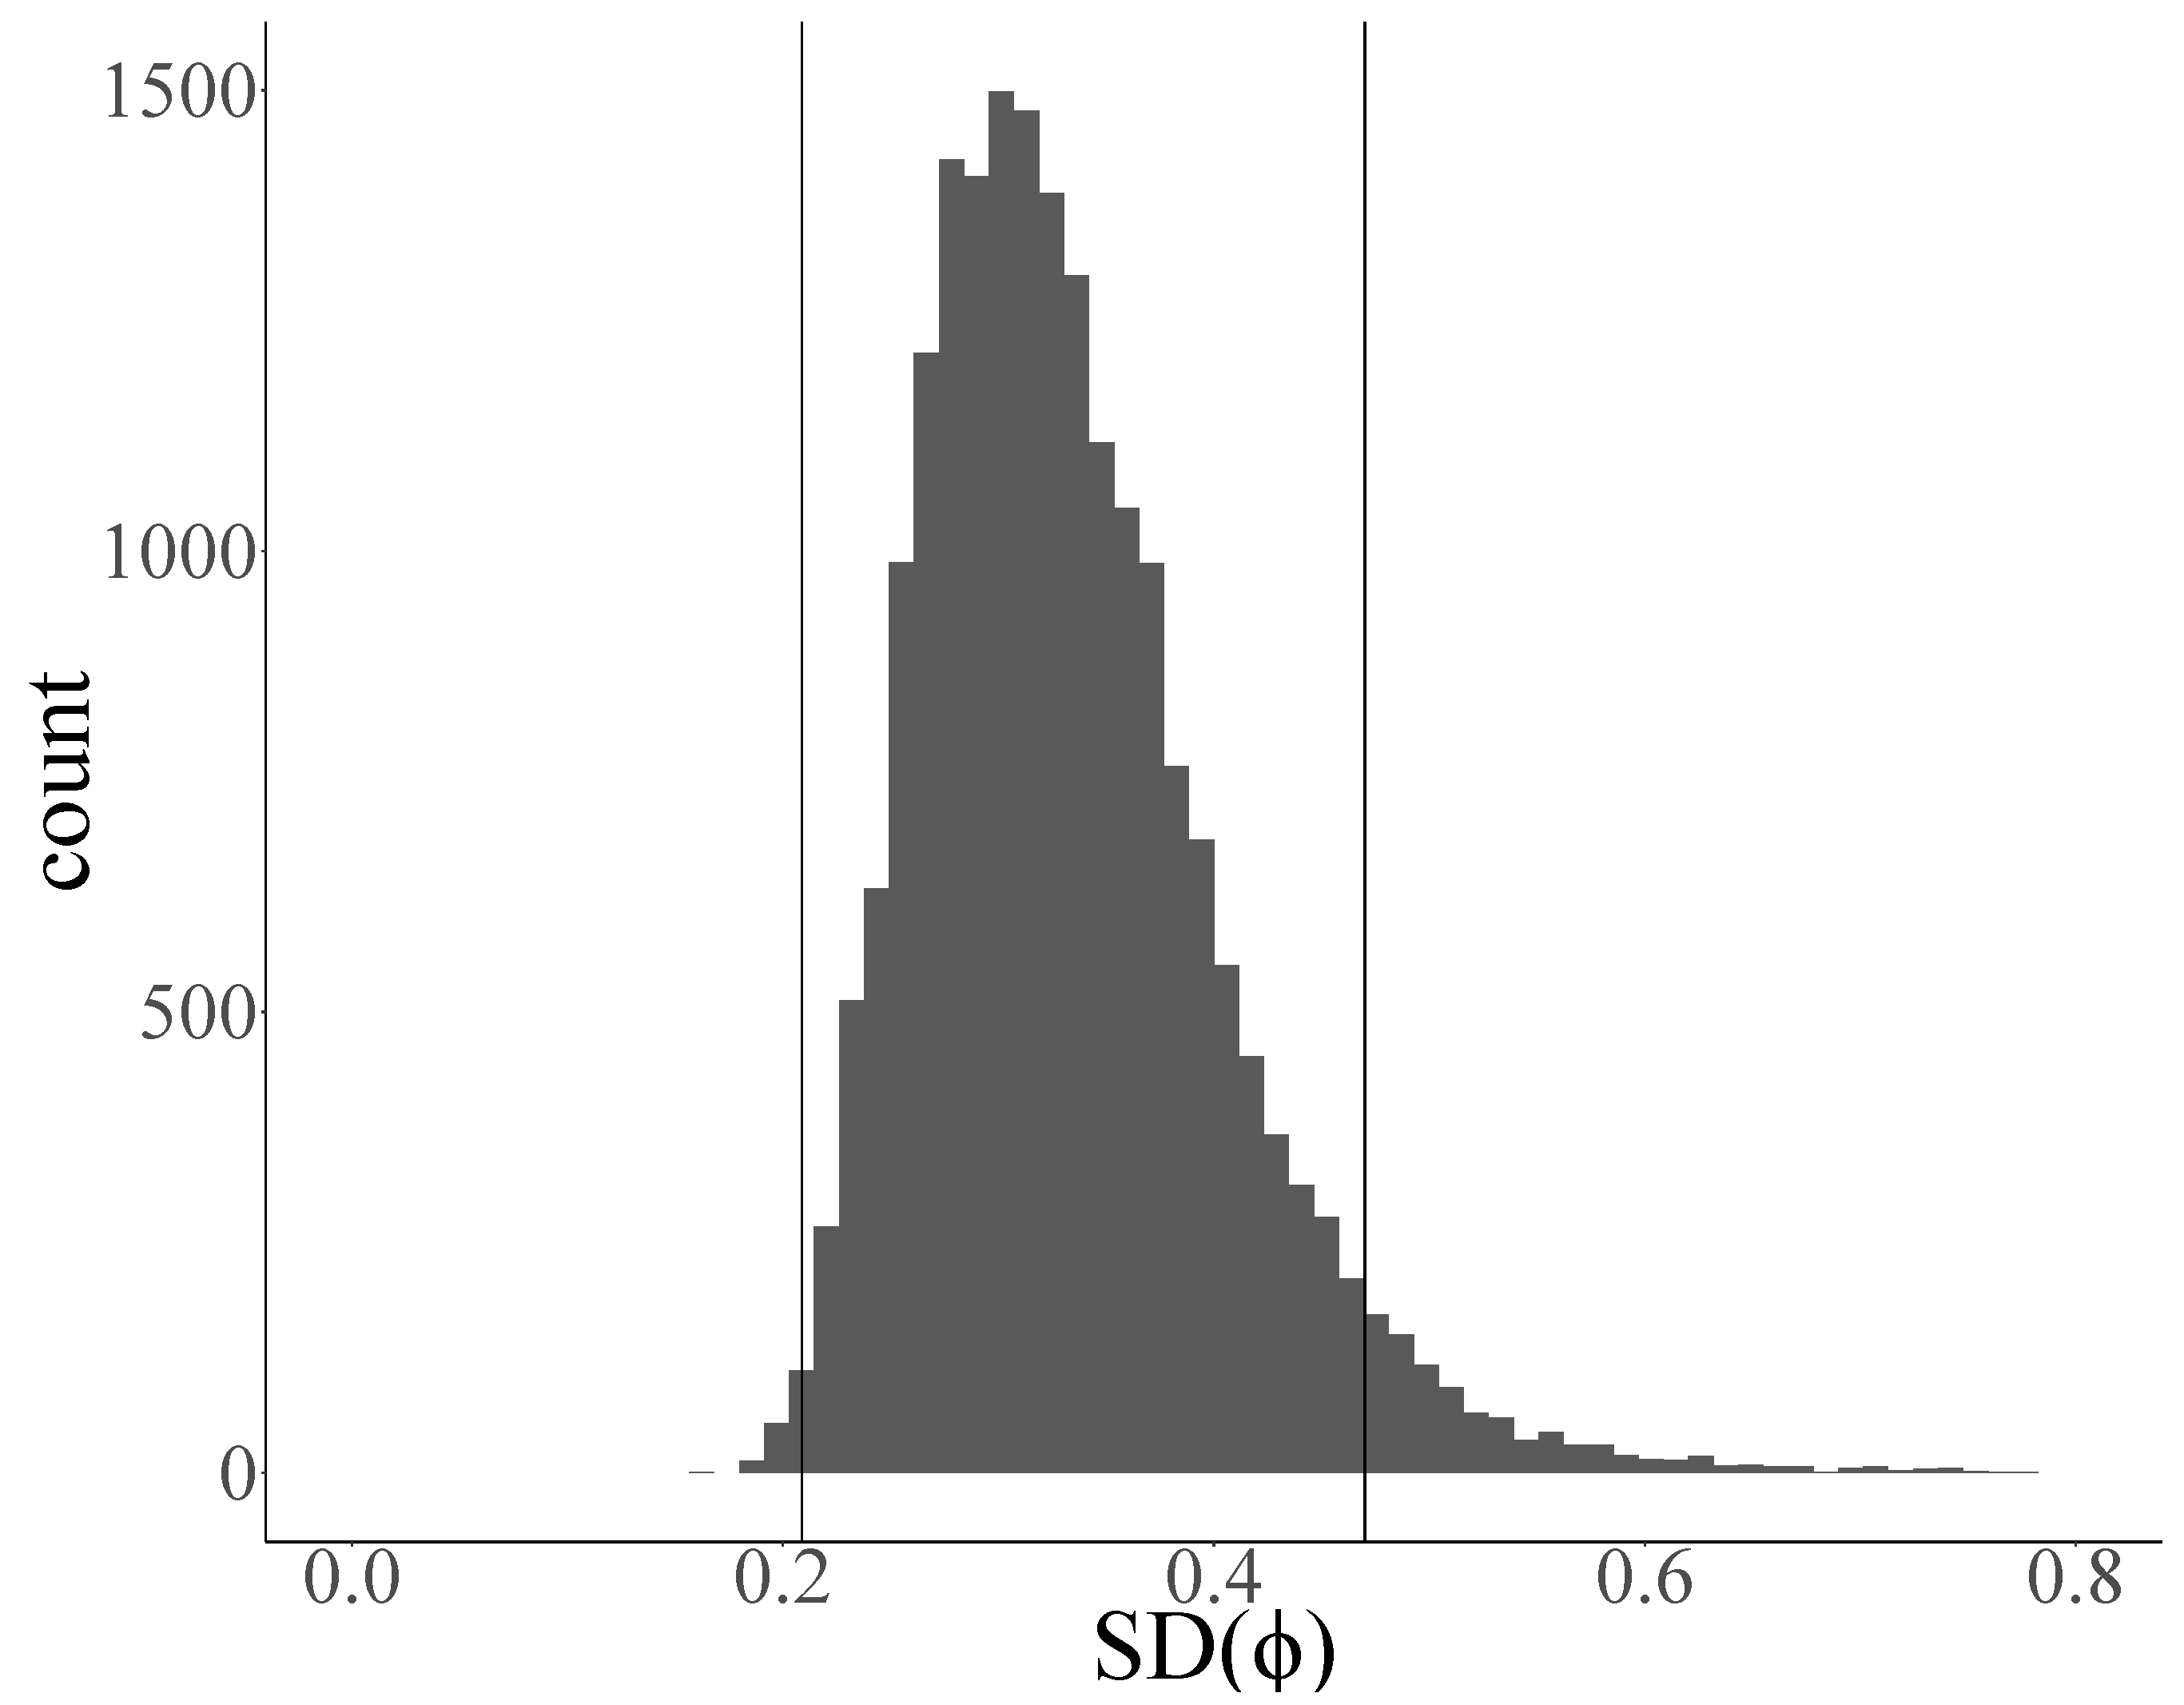
\includegraphics[height = 0.3\textheight]{phi_dist.eps}
	\end{center}
	\caption{Posterior distribution of the standard deviation of the speed sensitivity parameter $\phi_{k}$ across $j=12$ items.}
	\label{fig:post_phi}
\end{figure}

The complete posterior distribution of the standard deviation of $\phi_{k}$ is plotted in Figure \ref{fig:post_phi}. The Highest Posterior Density (HPD) interval, ranging from 0.21 to 0.47, excluded 0 and provides evidence that there was substantial variation in the speed sensitivity across items in the empirical data. 

Table \ref{tab:postCor} displays the means of the posterior distributions of the correlations among all item parameters. As expected, the time intensity and the difficulty parameter correlated positively ($r_{b_{k}  \lambda_{k}} = .25$), which is an often reported finding in the response time literature and has been extensively discussed in the context of adaptive testing \cite{vanderLinden.2013}. The speed sensitivity parameter $\phi_{k}$ was most strongly correlated with the time intensity parameter $\lambda_{k}$ with $r_{\phi_{k}  \lambda_{k}} = .21$. This implies that the speed sensitivity parameter was largely independent from the other item parameters and would not be indirectly balanced if the other item parameters were balanced between test forms.

\begin{table}[ht]
\centering
\caption{Means of the Posterior Distribution of Correlations Between the Item Parameters, j = 12.} 
\begin{tabular}{lllll}
  \hline
 & $b_{k}$ & $a_{k}$ & $\lambda_{k}$ & $\phi_{k}$ \\ 
  \hline
$b_{k}$ &  &  &  &  \\ 
  $a_{k}$ & 0.07 &  &  &  \\ 
  $\lambda_{k}$ & 0.25 & 0.27 &  &  \\ 
  $\phi_{k}$ & -0.05 & 0.12 & 0.21 &  \\ 
   \hline
\end{tabular}
\label{tab:postCor}
\end{table}

All analyses indicate that the assumption of the gHRT, namely that items differ regarding their speed sensitivity, is indeed justifiable. Additionally, the parameter seems to be rather independent from the other estimated parameters. All analyses results were replicated with a reading literacy booklet ('R01') and were found to be comparable. 

% ----------------------------- Simulation
\section{Simulation Study}
Using the findings and parameters distributions in the empirical analyses, a simulation study was conducted to investigate how severely differentially speed sensitive test forms influence ability estimation. 

\subsection{Design}
We created two test forms, each with 30 items. The item parameters for the first test form were drawn from a multivariate normal distribution as in Equation \ref{eq:gHRT_ItemMVN} with: 

\begin{equation}
	\mu_{I} = (\mu_{a} = 1.12, \mu_{b} = 0.54, \mu_{\phi} = 0.3, \mu_{\lambda} = 4.26)
\end{equation}
and
\begin{equation}
	\Sigma_I =	\begin{pmatrix}
\sigma^2_{a} = 0.45 &  &  &  \\
\sigma_{b, a} = 0.05 & \sigma^2_{b} = 1.00 &  &  \\
\sigma_{\phi, a} = 0.01 & \sigma_{\phi, b} = 0.03 & \sigma_{\phi}^2 = 0.01 &  \\
\sigma_{\lambda, a} = -0.02 & \sigma_{\lambda, b} = 0.13 & \sigma_{\lambda, \phi} = 0.01 & \sigma^2_{\lambda} = 0.25 \\
	\end{pmatrix}.	
\end{equation}

Means, variances and covariances of the item parameters were set to be in accordance with the results obtained from the empirical data analysis. $\phi_{k}$ and $a_{k}$ were censored at 0. If an item parameter draw included any $\phi_{k}$ and $a_{k}$ smaller than 0, all item parameters were drawn again for this replication. The residual variance of the log response times was drawn from a univariate normal distribution with $\sigma_{\epsilon_{k}} \sim \mathcal{N}(0.2, 0.1)$. This first test form, with $\mu(\phi_{k}) = 0.3$ is referred to as the \textit{low speed sensitivity test form}. 

The item parameters of the second test form were identical to the item parameters of the first test form except for the speed sensitivities $\phi_{k}$, which were shifted by $ + 0.4$. This second test form is referred to as the \textit{high speed sensitivity test form}, with $\mu(\phi_{k}) = 0.3 + 0.4 = 0.7$. Person parameters were chosen to enable conclusions about the effect of the two differing test forms on all possible combinations of speed and ability. Therefore we sampled 500 ability parameters from $\theta_{i} \sim \mathcal{N}(0, 1)$ and combined these with four different levels of speed, $\zeta_{i} = [-1; -0.5; 0.5; 1]$. This resulted in a complete sample of $n = 2000$ test takers across the four speed subgroups. 

We simulated responses and response times of the complete sample working on both test forms according to the gHRT. We set the time limit to 65 minutes and scored all responses for which the cumulative response time was greater than this limit as incorrect. This time limit was chosen to introduce a reasonable amount of not reached items into the simulation given the number of items and the respective item time intensities. Overall, 500 replications were conducted. 

\subsection{Methods}
Responses were analyzed via the 2PL IRT model using the R package TAM \cite{Robitzsch.TAM}. Difficulties $b_{k}$ and discriminations $a_{k}$ were treated as known, as if they were obtained in a previously conducted calibration study. Person parameters were estimated using the weighted likelihood estimator (WLE) \cite{Warm.1989}. We compared numbers of not reached items for the four different speed groups between the two test forms. Furthermore we investigated the estimated abilities compared to the true abilities in all subgroups between the two test forms.

\subsection{Results}
\begin{figure}	[!htb]	
	\begin{center}
		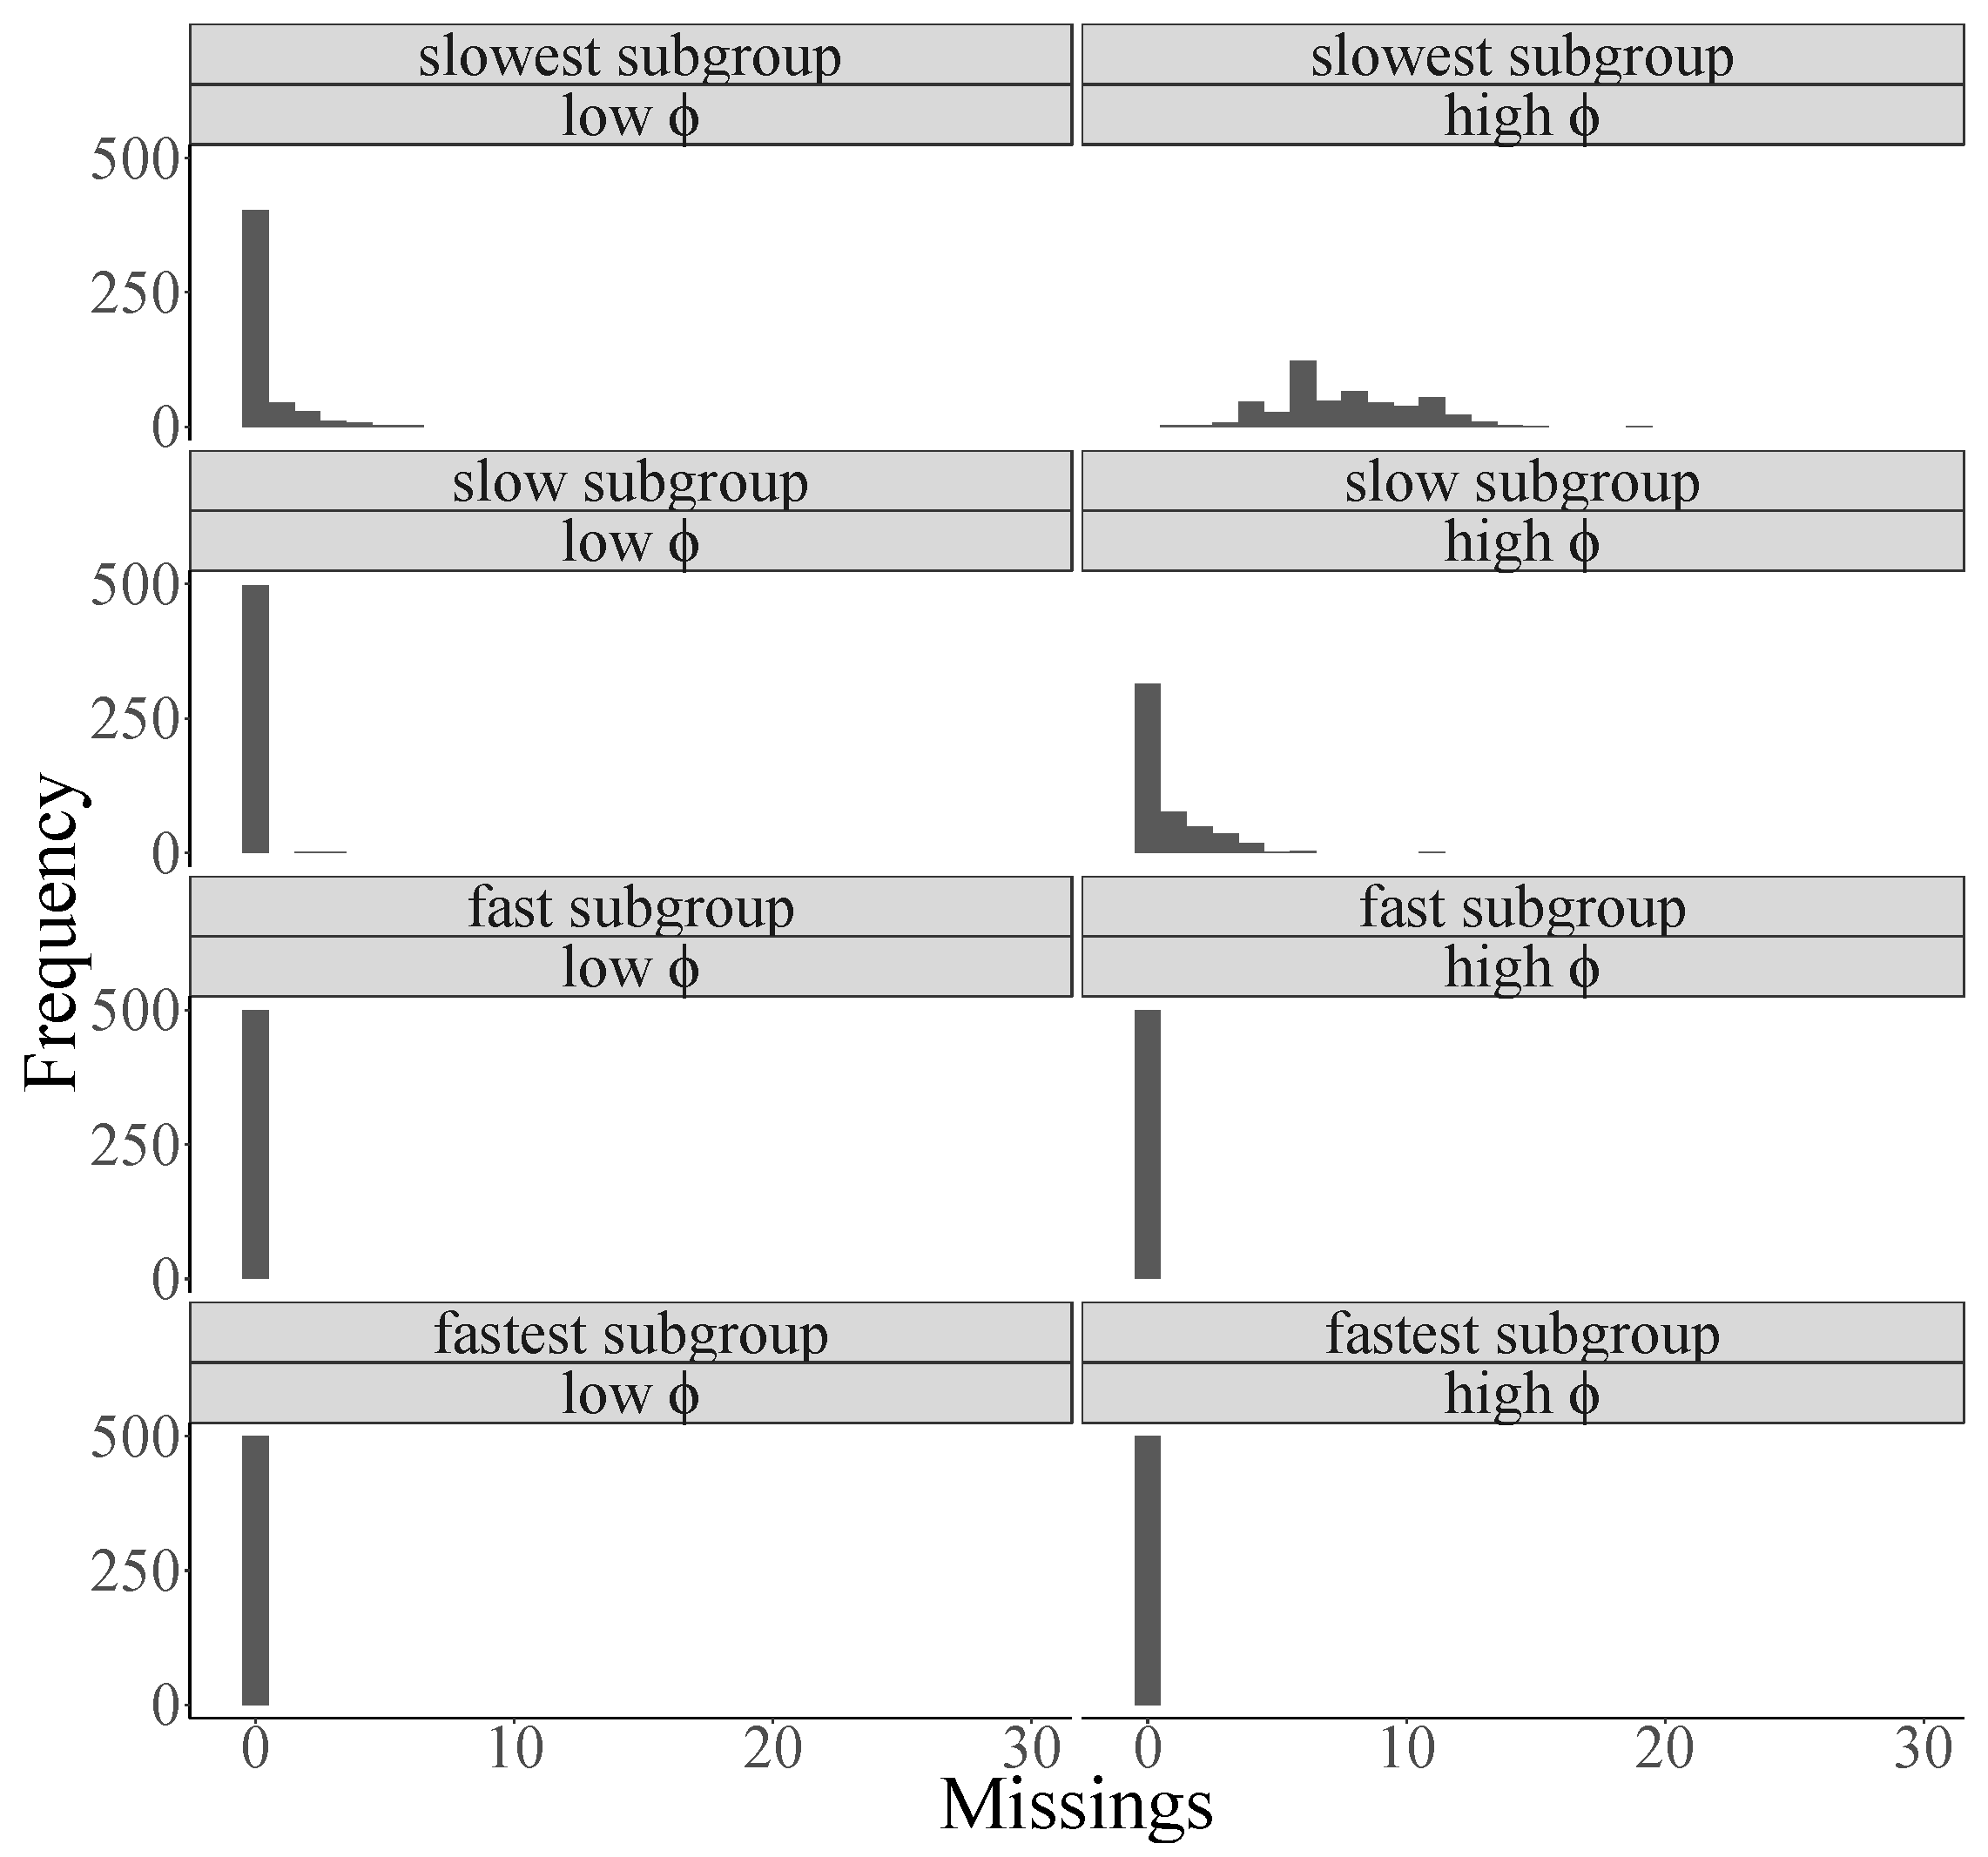
\includegraphics[height = 0.4\textheight]{miss_subGroup.eps}
	\end{center}
		\caption{Number of not reached items for the low and high speed sensitivity test form, across the four subgroups. Results shown for a randomly selected single replication.}	
		\label{fig:miss}
\end{figure}

As can be predicted from the response time measurement model in Equation \ref{eq:gHRT} and the response time characteristic curves in Figure \ref{fig:phi_theoret}, differences in cumulative response times between the two test forms were most severe for the fastest and slowest participants.  In the faster subgroups, the differences in testing time did not result in different numbers of not reached items, because for both test forms the testing times were well below the time limit. For the slowest participants, however, the high speed sensitivity test form led to substantially more not reached items than the low speed sensitivity test form (Figure \ref{fig:miss}). 

These differences in number of not reached items also resulted in differences in ability estimates. The average difference in ability estimation between the test forms for the slowest subgroup was 0.52 (see Table \ref{tab:bias}), with the high speed sensitivity test form resulting in substantially lower ability estimates. This difference in the ability logit is equal to, for example, a drop from the 50th ability percentile (the person scores higher or as high as 50 percent of the population on the test) to the 32th ability percentile (the person scores higher or as high as 32 percent of the population on the test). For all other speed levels, in contrast, there was either no bias or the bias was negligible. 

\begin{table}[ht]
\centering
\caption{Analysis of Bias in Person Parameter Estimation and Differences in Bias Between Booklets for Speed Subgroups, Averaged Across All Replications.} 
\begin{tabular}{lrrr}
  \hline
Speed & low $\phi$ & high $\phi$ & Diff \\ 
  \hline
slowest & -0.04 & -0.56 & 0.52 \\ 
  slow & 0.00 & -0.06 & 0.06 \\ 
  fast & 0.00 & 0.00 & 0.00 \\ 
  fastest & 0.00 & 0.00 & 0.00 \\ 
   \hline
\end{tabular}
\label{tab:bias}
\end{table}

However, differences in ability estimation were not homogeneous within the slowest subgroup. Especially participants with high ability had substantially different ability estimates depending on the test form (see the upper left graph in Figure \ref{fig:abil}). This was to be expected, because for slow but high ability test takers there are many not-reached items (scored as incorrect) that they could have answered correctly under sufficient time conditions. This is not the case for slow and low ability test takers, which demonstrated only minor differences in estimated ability across the test form.

\begin{figure} [!htb]	
	\begin{center}
		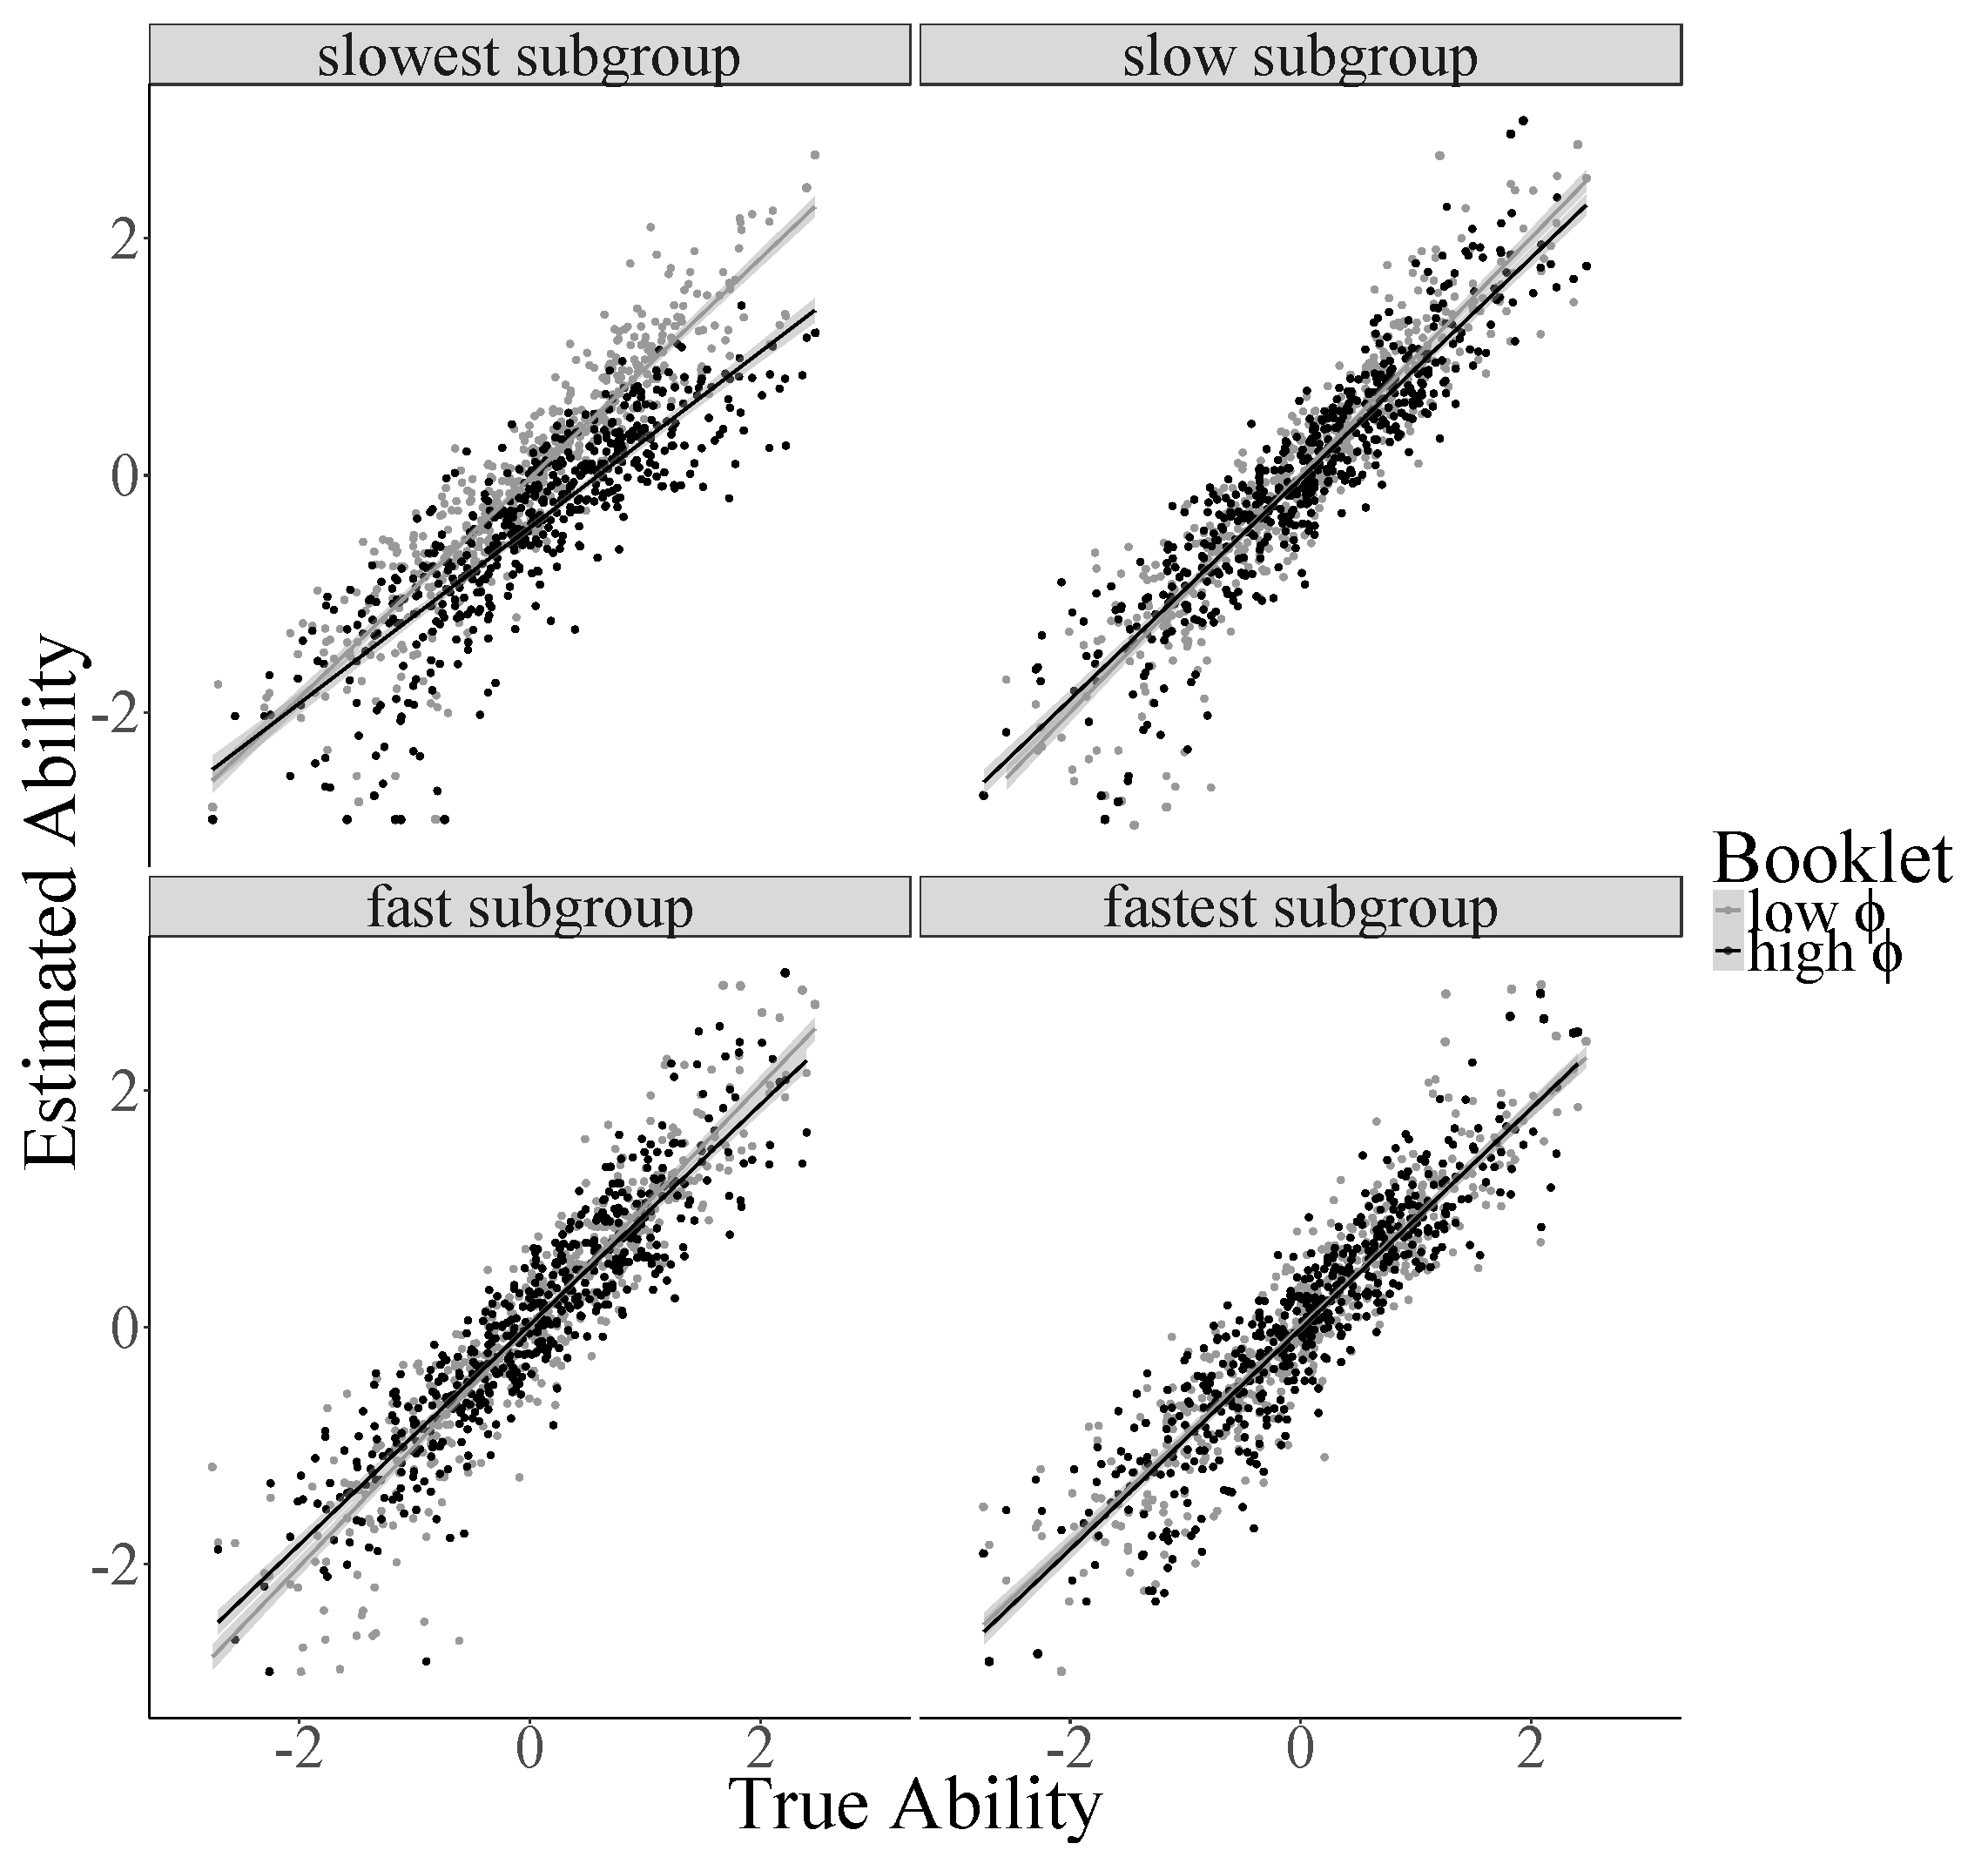
\includegraphics[height = 0.4\textheight]{abil_subGroup.eps}
	\end{center}
		\caption{True and estimated ability for the low and high speed sensitivity test form, across the four subgroups. Results shown for a randomly selected single replication.}	
		\label{fig:abil}
\end{figure}

Table \ref{tab:descr} shows more detailed test descriptive statistics per speed level and per test form. Noteworthy are the differences between the mean cumulative response times (denoted as $RT_{tot}$) for the different speed levels. The fast participants were much faster than the time limit of 3900 seconds, with means of 1309.45 seconds and 1954.34 seconds for the high and the low speed sensitivity test forms. In contrast, especially the slowest subgroup working on the high speed sensitivity test form was, on average, substantially slower than the time limit, with a mean of 5419.48 seconds. 

The root mean square error (RMSE) indicates the measurement precision of an estimate and is defined as 
\begin{equation}
	\textrm{RMSE} = \sqrt{\frac{\sum_{i = 1}^{n} (\widehat{\theta_i} - \theta_i)^2}{n}}.
\end{equation}
For the high speed sensitivity test form the RMSE in the slowest group ($\textrm{RMSE} = 0.84$) was about twice as high as in the other groups. No such difference was found for the low speed sensitivity test form. Furthermore, the correlation between estimated and true ability considerably dropped for the slowest subgroup working on the high speed sensitivity test form ($r_{\theta_{true} \theta{est}} = .82$).

To conclude, the simulation shows that differences in speed sensitivity between test forms can lead to substantial differences in ability estimates especially for slow and able test takers. This finding is independent from whether speed is seen as a nuisance parameter or part of the construct to be measured. Furthermore, if speed is seen as a nuisance parameter, the high speed sensitivity test forms leads to a more biased and less precise ability measurement. 
 
\begin{table}[ht]
\centering
\caption{Test Statistics per Test Form and per Speed Group, Averaged Across All Replications.} 
\begin{tabular}{llrrrrrr}
  \hline
Test Form & $\zeta_{i}$ & $M(RT_{tot})$ & $SD(RT_{tot})$ & $M(Mis)$ & $SD(Mis)$ & $cor(\theta_{true} \theta_{est})$ & RMSE \\ 
  \hline
low $\phi$ & slowest & 3634.74 & 367.96 & 0.02 & 0.04 & 0.90 & 0.47 \\ 
  low $\phi$ & slow & 3100.20 & 312.82 & 0.00 & 0.01 & 0.91 & 0.45 \\ 
  low $\phi$ & fast & 2273.33 & 227.33 & 0.00 & 0.00 & 0.91 & 0.45 \\ 
  low $\phi$ & fastest & 1954.34 & 196.28 & 0.00 & 0.00 & 0.91 & 0.45 \\ 
  high $\phi$ & slowest & 5419.48 & 551.18 & 0.30 & 0.09 & 0.82 & 0.84 \\ 
  high $\phi$ & slow & 3785.80 & 382.40 & 0.03 & 0.06 & 0.90 & 0.48 \\ 
  high $\phi$ & fast & 1861.38 & 186.27 & 0.00 & 0.00 & 0.91 & 0.45 \\ 
  high $\phi$ & fastest & 1309.45 & 131.00 & 0.00 & 0.00 & 0.91 & 0.45 \\ 
   \hline
\end{tabular}
\begin{tablenotes}
\vspace{0.1cm}
\small
    \textit{Note:} Descriptive statistics are depicted for mean response times M($RT_{tot}$) and the corresponding standard deviation SD($RT_{tot}$), mean amount of missings M(Mis), the corresponding standard deviation SD(Mis), correlation between true and estimated ability $cor(\theta_{true} \theta_{est})$ and root mean square error (RMSE). 
\end{tablenotes}
\label{tab:descr}
\end{table}

% ----------------------------- Discussion
\section{Discussion}
High-stakes assessments often require multiple test forms with equal speededness at the level of the test taker. So far, the use of average response times and the use of the hierarchical response time model by \citeA{vanderLinden.2006} have been proposed as strategies to control speededness across test forms. Although these approaches can constrain the expected average testing time to be equal across test forms, they rely on the strong assumption that all items are equally sensitive to differences in speed levels across test takers. 

We investigated whether this assumption is violated in empirical data using the generalized hierarchical response time model \cite{Fox.2007, KleinEntink.2009}, which models these differences in speed sensitivity. The gHRT fitted the data better than the HRT and the speed sensitivity parameter substantially varied across items. This means that balancing test forms using either observed response times or the HRT can indeed lead to unbalanced speed sensitivity across test forms. Furthermore, the speed sensitivity parameter was only slightly correlated with other item parameters. This implies that, if one would balance the test forms using only the other item parameters, there is no guarantee that the test forms will be balanced with respect to speed sensitivity.

Moreover, when missing responses are treated as incorrect (a standard practice in high-stake assessments) differences in speed sensitivity can result in differences in the ability estimates across test forms for specific test takers. We investigated the severity of bias in a simulation study based on the results of the empirical analysis. Our results show that differences in speed sensitivity between test forms can lead to substantial differences in ability estimation, due to increased numbers of not reached items. Especially slow test takers with high ability were affected. 

Therefore, we draw the following conclusions regarding the practice of assembling test forms for educational high-stakes assessments: Right now, the use of the HRT is the state of the art approach when balancing test forms. However, our findings suggest that only when 
\begin{seriate}
\item the HRT proves to better fit the data than the gHRT or 
\item the gHRT shows low variation in the speed sensitivity parameter across items,
\end{seriate}
the HRT should be considered sufficient. Model comparisons can be conducted using the DIC \cite{Spiegelhalter.2002}. If the gHRT shows better model fit and speed sensitivity varies substantially across items, the gHRT should be used when calibrating the items. For test assembly, all freely estimated parameters on the item level (item time intensity, speed sensitivity, residual variance of the response times) should then be balanced across test forms. 

The issue of differential speed sensitivity can also be illustrated from an alternative perspective: As stated before, we assume that high-stakes tests usually are speeded power tests and therefore that the ability measured in the test is a composite measure of ability and speed. However, this composition changes between test forms if there are differences in speed sensitivity between test forms. If a test form has a high speed sensitivity and a time limit induces time pressure for reasonable speed levels, the proportion of speed in the composite measure can be considered quite high. If in the same scenario a test form has low speed sensitivity, however, the proportion of speed in the composite measure for this test form is rather low. We argue that, for high-stake assessment, the influence of speed on the ability estimation has to be the same across test forms. 

To deal with differences in speed sensitivity across items, applying the gHRT and balancing speed sensitivity when assembling test forms is not the only possible strategy. For instance, one could assume that all problems regarding differential speededness of tests could be avoided when tests are designed to be unspeeded, that is, without any time pressure for all test takers. Because in most educational assessments speed is a nuisance parameter that is conceptually not part of the construct being measured, this strategy seems promising. In practice, however, designing unspeeded tests appears to be unfeasible. The average testing times of the simulated data in Table \ref{tab:descr} show that when test takers differ in working speed, this can lead to substantial differences in required testing time for longer tests. Similar results are reported by \citeA{vanderLinden.2013}, who also used empirically-based simulated data. Assuring that even the slowest test takers can work without time pressure would imply a time limit that is far too generous and problematic both from an economical perspective (e.g. expensive testing time on computers) as well as from a motivational perspective (faster test takers waste their time). Hence, completely unspeeded testing situations seem impossible in practice. 

Based on our findings we also argue that investigating whether a test is unspeeded or not can be rather challenging: To assess the speededness of a test, frequently experimental methods using different time limits or different numbers of items in the same time limit have been used \cite<e.g.>{Bridgeman.2004GRE,Bridgeman.2004SAT,Harik.2018}. Our findings indicate that these methods of comparing average ability estimation between experimental conditions to assess the speededness of a test have important limitations. For the majority of the test takers more generous time limits might only have a small impact on the demonstrated ability. However, different time limits can still substantially affect the slowest part of the population, an effect that can only be disentangled by explicitly modeling speed. If differences in ability estimation for different time limits are averaged over all test takers or calculated for different ability levels, the degree of speededness of the test for slow test takers could be severely underestimated. Therefore, tests that have been examined using the aforementioned methods could have been falsely classified as unspeeded. 

\subsection{Limitations and Practical Implications}
There are a number of limitations to our study: First, our real data analyses are based on low-stakes data while implications are mainly relevant for high-stakes assessments. However, similar analyses on (non-educational) high-stakes data show results comparable to our study \cite{Fox.2017}. Furthermore, we do not conclude that the gHRT will always demonstrate better model fit than the HRT for item pools of high-stakes assessments. However, we argue that the assumption of equal speed sensitivity across items (cf. HRT) is very strong, and should be tested, just like the assumption of equal factor loadings should be tested in confirmatory factor analysis or structural equation modeling \cite[pp. 236-252]{Brown.2006}. Additionally, to obtain unbiased item parameters, we recommend to pilot items for high-stakes assessments under low-stakes conditions.

A second, important limitation of the gHRT is its strong assumption of conditional independence between responses and response times. This means that, given the common distribution of the person and item parameters, the model assumes uncorrelated residuals. This assumption is violated, if participants substantially speed up or slow down during the test. This could very well happen in high-stakes assessments with a time limit, as test takers might speed up if they feel they are running out of time. While the estimation of person parameters will be strongly affected if the conditional independence assumption is violated, item parameters can be assumed to be less affected. Indeed, for test assembly purposes only item parameters and their relations across items are of interest. Nevertheless this has important consequences for the design of pilot studies of high-stakes assessments. For the purpose of well estimated item parameters for the speed model, not too tight time limits seem beneficial, because this lets most of the participants work at their maximum ability. If participants speed up on items or guess on items, item parameters estimates will either be more imprecise (if position effects are controlled for) or biased (if position effects are not controlled for). To control for item position effects on the response times, similar methods can be applied, as when controlling for position effects of ability item parameters estimation \cite<e.g.,>{Gonzalez.2010}. Of course, these methods assume that all items parameters are all equally effected by position effects. Avoiding speeding up seems easiest, if items were piloted in low-stakes settings. However, under these conditions motivational issues might effect item parameter estimation as well.

\subsection{Outlook}
While our study shows that not incorporating the gHRT and its speed sensitivity parameter in the item calibration and test assembly can lead to biased ability estimates, the question how the parameter should be incorporated in the test assembly process has not been answered yet. Furthermore, in the past, automated test assembly procedures have been developed to enable the fast assembly of multiple test forms from large item pools under various constraints \cite{vanderLinden.2005}. These methods are already frequently used in practice \cite<for an overview of assessments using these approaches, see>{Luecht.2011}, using observed response times or the HRT. To enable the use of the HRT in automated test assembly, \citeA{vanderLinden.2011reparamet} reparameterized the model for constraining in the test assembly process. He showed that it is possible to constrain the speededness in a mixed integer programming model \cite{vanderLinden.2011ATA}. Future research should investigate if a similar reparameterization can be performed for the gHRT to be used in automated test assembly. 

Although we focused on high-stakes testing, our findings may also have implications with respect to low-stakes assessments. In low-stakes assessments the practice of scoring not reached items as incorrect has received lots of critisism. Rather than scoring them as incorrect, missing responses are frequently ignored when estimating ability \cite{Pohl.2013}. When applying this strategy to our simulated data, we did not find any bias regarding the ability estimation. However, the differences in RMSE remained: RMSE was increased for slower test takers for the high speed sensitivity test form. However, even if missings were scored incorrect in large-scale assessments, the resulting bias would cancel out if only group-level results are reported and if speed distributions are identical between groups. But even in these cases, taking into account the speed sensitivity of items can have a beneficial impact, because measurement accuracy can be enhanced by balancing time intensive and speed sensitive items evenly across test forms. 

Finally, the gHRT approach could also be useful to determine the speededness of assessments under various time constraints for different test taker populations without having to experimentally investigate all possible combinations. This would especially be valuable for determining test accommodations for students with disabilities \cite{Lovett.2010}. Furthermore, while the current paper focuses on fixed-test forms, our findings can also be applied to computerized adaptive testing or multistage testing. Studies haven shown that differential speededness of test forms is an even greater challenge in these settings \cite{vanderLinden.2013}. Investigating, whether the gHRT could contribute to the fairness of these assessments, seems worthwhile as well.

% ----------------------------- References
\begin{flushleft}
\bibliography{references}
\end{flushleft}


\end{document}